\documentclass{beamer}

% Preamble
\usetheme{Copenhagen}
\usecolortheme{seagull}
\usefonttheme[onlysmall]{structurebold}
\setbeamerfont{title}{shape=\itshape,family=\rmfamily}
\setbeamertemplate{footline}[frame number]
\usepackage[absolute,overlay]{textpos}
\useinnertheme{circles}
\usepackage{tikz,overpic}
\usepackage{verbatim}
\usetikzlibrary{fit,shapes.misc,arrows}
\usepackage{varwidth}


\usepackage{verbatim}
\usetikzlibrary{arrows,shapes}

% put the text at the right corner
\newcommand\FrameText[1]{%
  \begin{textblock*}{\paperwidth}(0pt,\textheight)
    \raggedright #1\hspace{.5em}
  \end{textblock*}}


% title page
\title{Bayesian Network of Targeting Interactions in Chromatin: Reanalyzed}
\author{Ricky Lim \\ \texttt{Ricky.lim@student.uva.nl}}
\date{\texttt{
 June 26, 2012\\
 Interdisciplinary Seminar on Biological Networks}
}
\institute{
 Universiteit van Amsterdam\\
 Faculty of Science\\
 Biomedical Sciences
} 

% start the frames
\begin{document}

\frame{\titlepage}
  
  
\frame
{
  \frametitle{Outline}
  \tableofcontents[pausesections]
}




\section[Introduction]{Introduction}
\subsection{Chromatin:Revisited}
\frame
{
 \frametitle{Chromatin:Revisited}
  \begin{figure}
   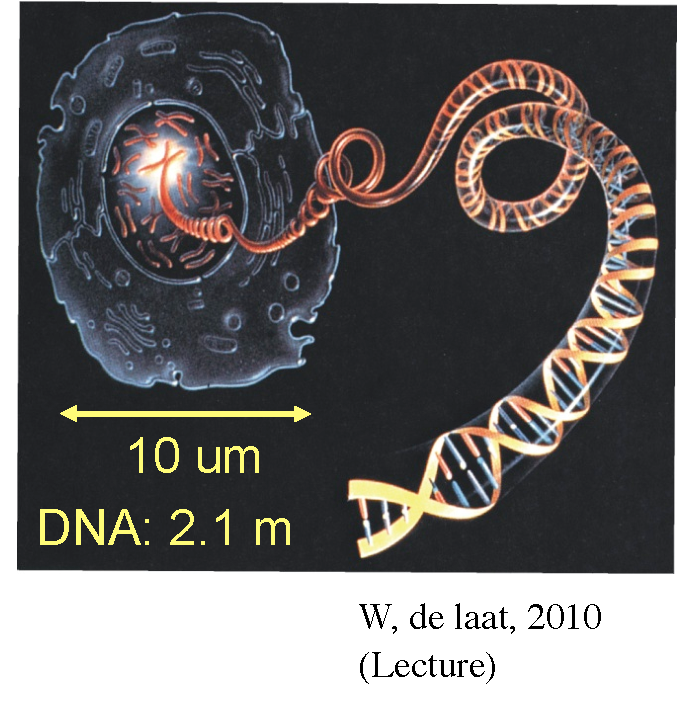
\includegraphics[width=.35\textwidth]{figures/dnasize.pdf}
   \pause
   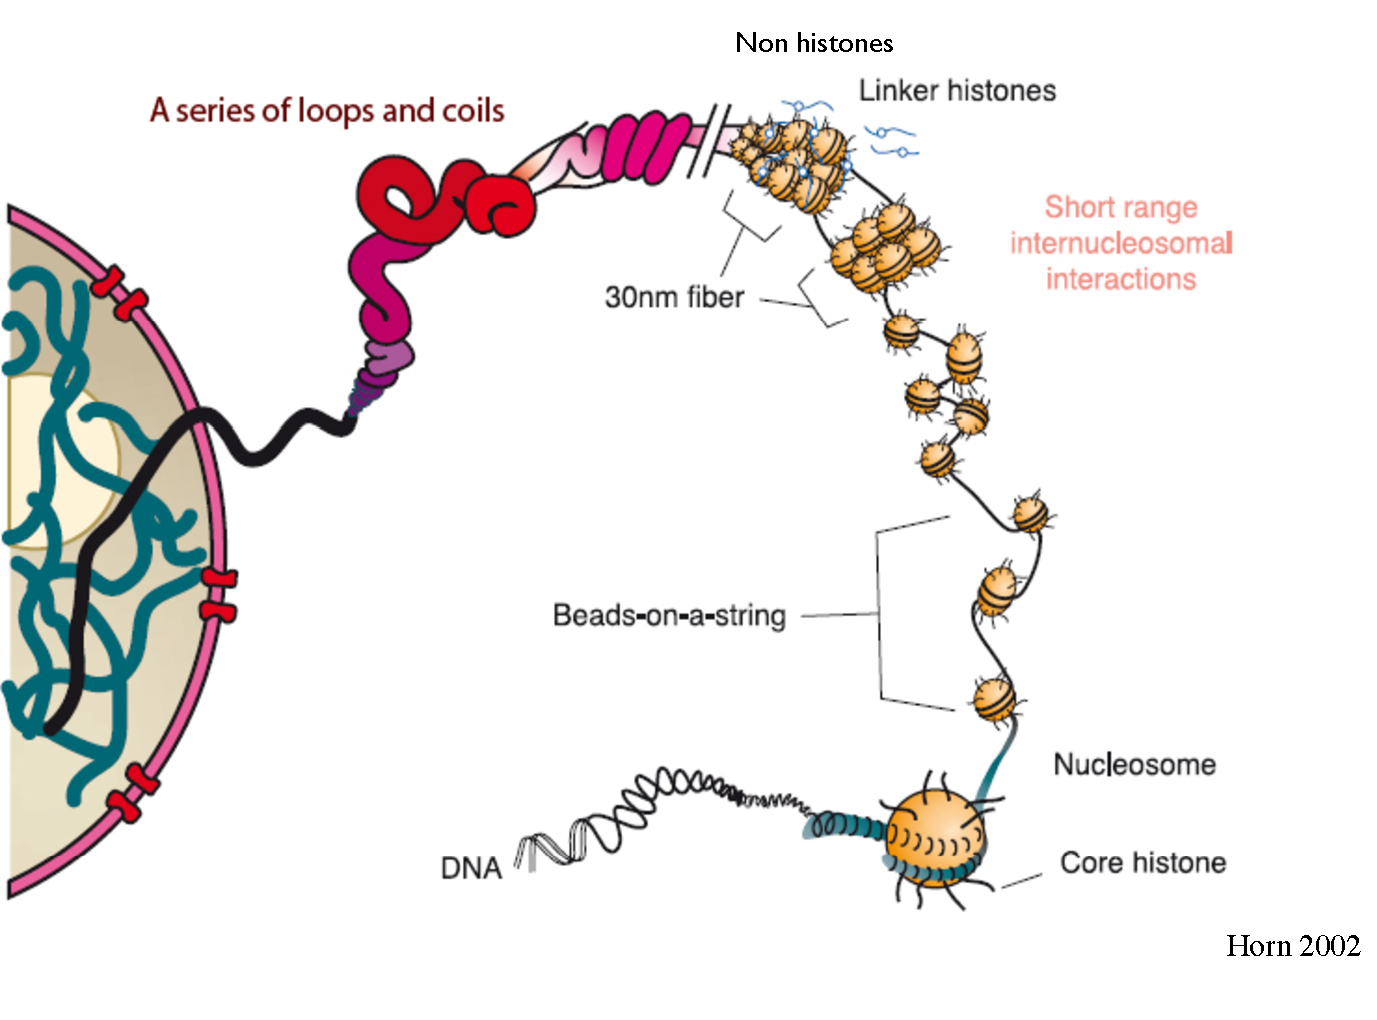
\includegraphics[width=.65\textwidth]{figures/folding.pdf}
  \end{figure}
  \pause 
  \alert{Chromatin} is a complex consisting of DNA, histones, and non-histones proteins(Chromatin Components)
}

\frame
{
 \frametitle{Main Players in Chromatin}
 \begin{figure}
  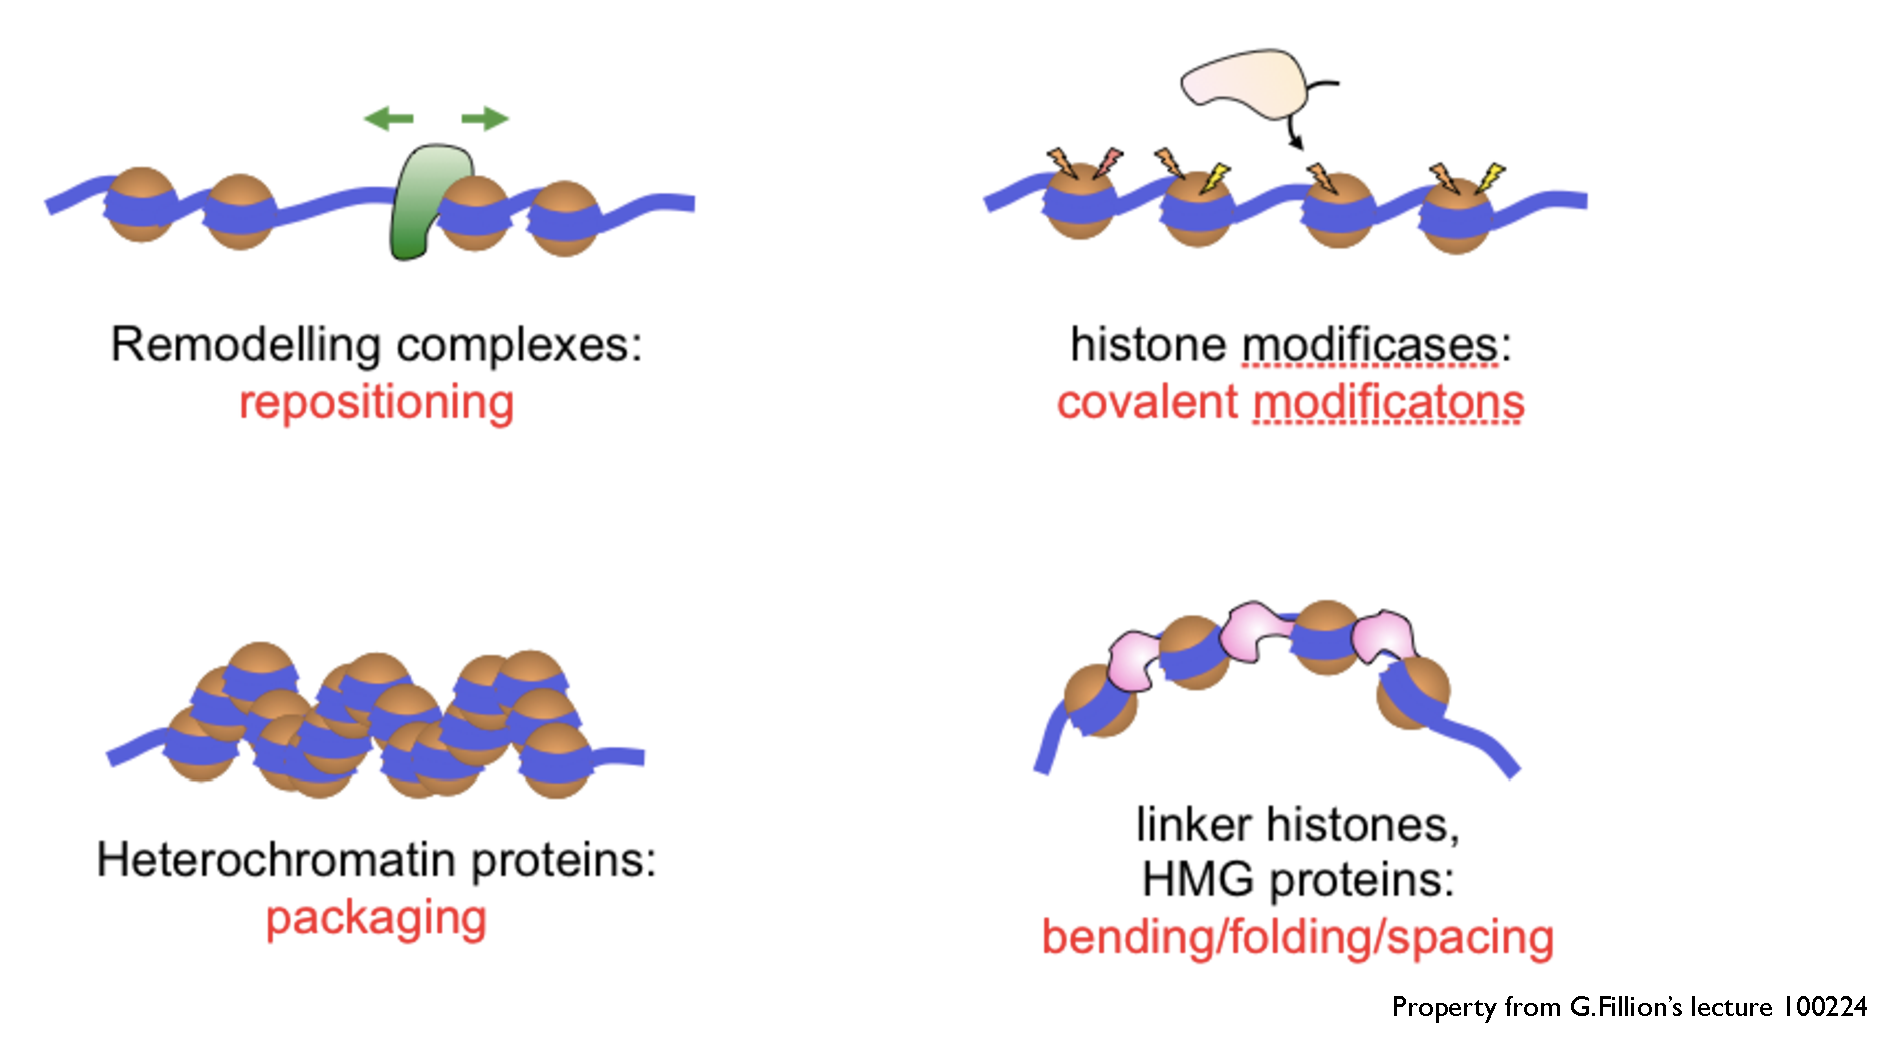
\includegraphics[width=1.10\textwidth]{figures/chromoplayers.pdf}
 \end{figure}
}

\subsection{Targeting Interactions in Chromatin}
\frame[label=map]
{
  \frametitle{Where Are These Players located ?}
   \begin{center}
     \begin{tikzpicture}
      \node<2->[anchor=south west,inner sep=0] at (0,0) {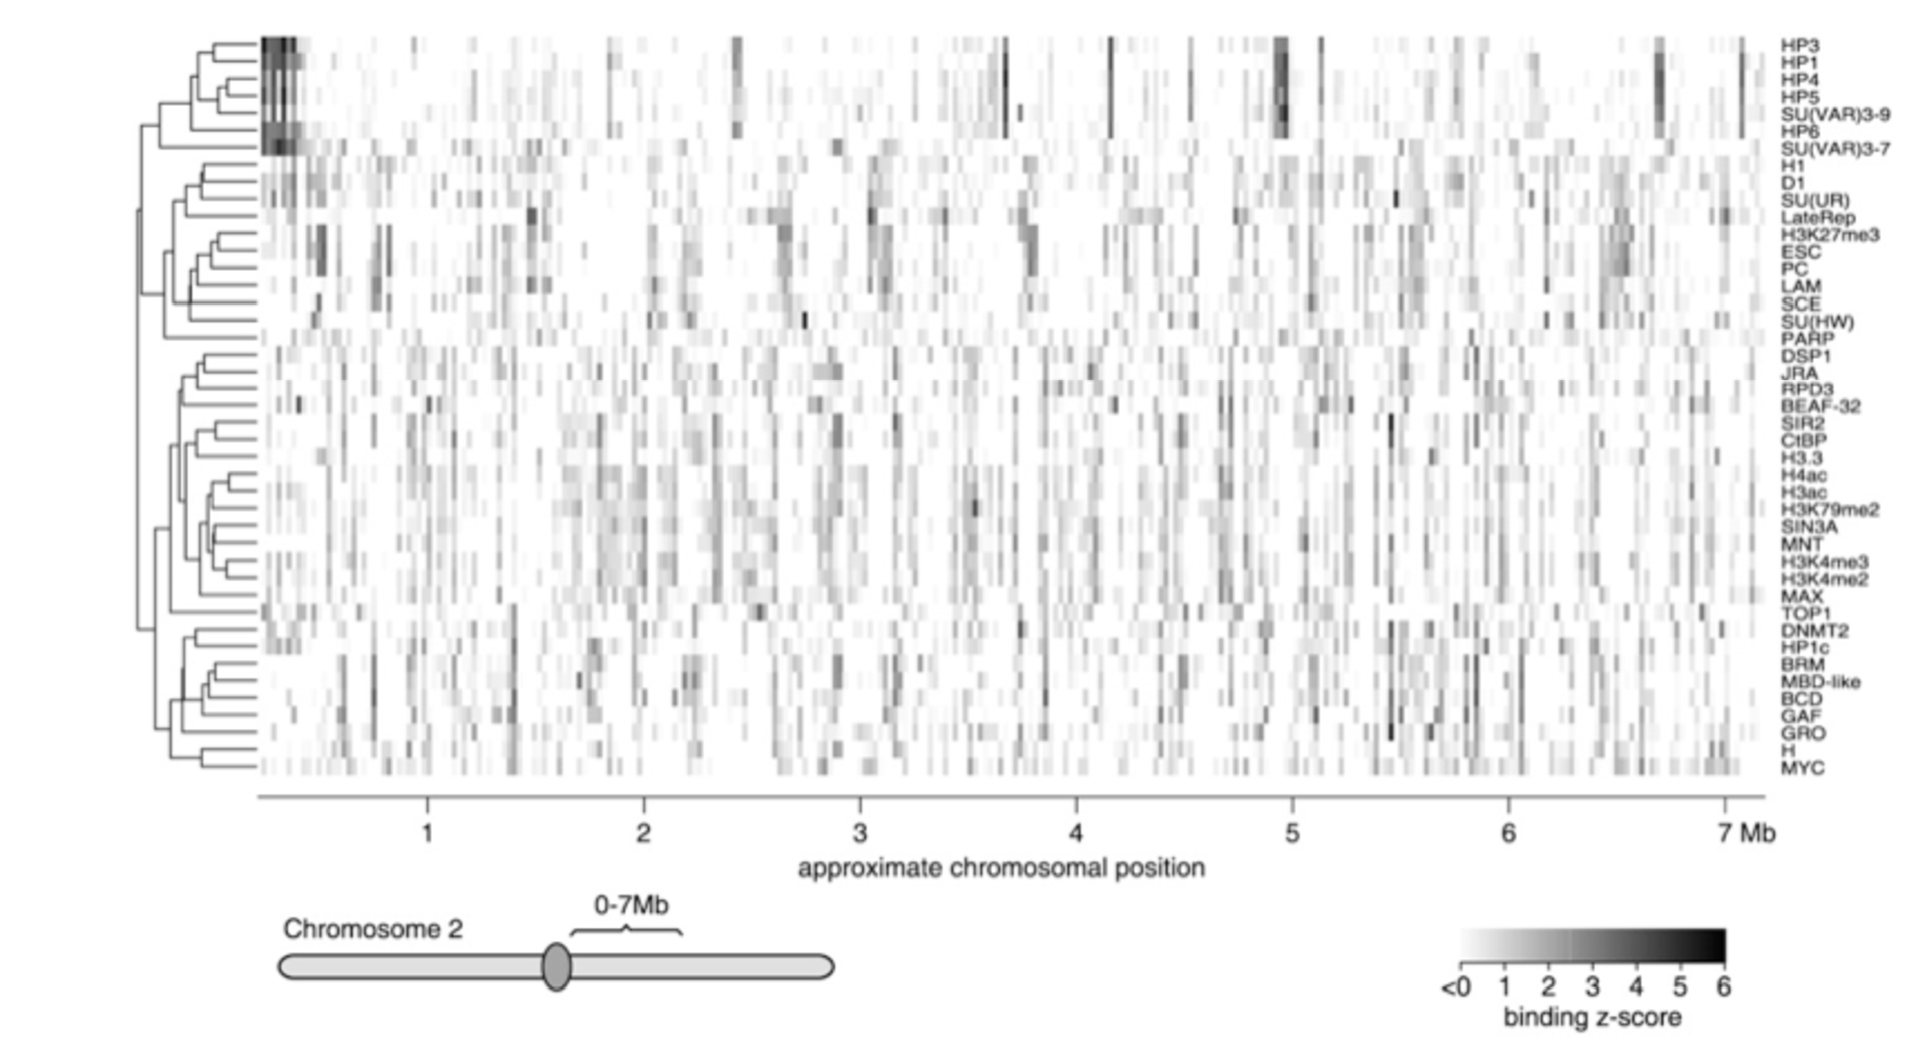
\includegraphics[width=1.3\textheight]{figures/43map.pdf}};
      \draw<3->[red,ultra thick,rounded corners] (1.4,5.3) rectangle (10.7,5.9);
      \draw<4->[red,ultra thick,rounded corners] (1.4,4.35) rectangle (10.7,4.75);
          
     \end{tikzpicture}
     \only<5>{\alert{Genome-wide specific binding patterns of components.}}  
       
   \end{center}
     

  
  \FrameText{\hfill\hyperlink{damid}{\beamerbutton{DamID}}}
  
}



% define simple flow chart
\tikzstyle{block} = [rectangle, draw, fill=gray!20, 
    text width=\textwidth, text centered, rounded corners, minimum height=4em]
\tikzstyle{line} = [draw, -latex']

\frame
{
  \frametitle{What determines the specific locations ?}
  
  % chart
  \begin{tikzpicture}[node distance = 2cm, auto]
    % Place nodes
    \node [block] (hypothesis) {\alert{Hypothesis:}\\ By the interactions among the chromatin components};
    \pause
    \node [block, below of=hypothesis] (network) {Network of Targeting Interactions};
    \path [line] (hypothesis) -- (network);
    \pause
    \node [block, below of=network] (approach) {1. Comparing the Binding Maps\\2. Systematic Search using Bayesian Network Analysis };
    \path [line] (network) -- (approach); 
   
    
  \end{tikzpicture}
}
  



\subsection{Bayesian Network(BN):Revisited}
\frame
{
  \frametitle{Bayesian Network(BN):Revisited}
  \textbf{Background:}
  \begin{itemize}[<+->]
   \item {a model of dependencies between multiple components of a system}
   \item {\alert{Assumption: Most components are (conditionally) independent of each other}}
  \end{itemize}
  \pause
  \begin{figure}
   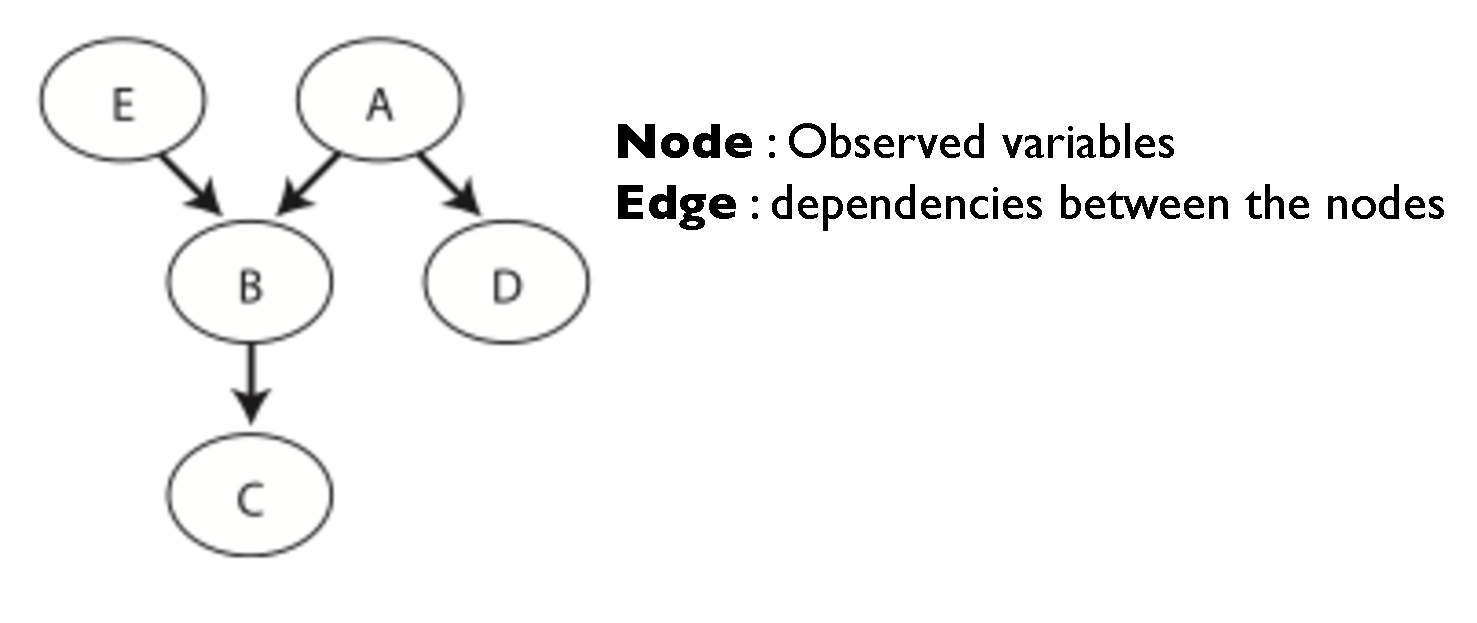
\includegraphics[width=.9\textwidth]{figures/BN.pdf}
  \end{figure}
  \FrameText{\small{\hfill{Pe�er, 2005}}}
}
  
  
  
\frame[plain]
{
  \frametitle{Learn BN of Targeting Interactions from Scratch}
   Problem Statement:\\
  \begin{itemize}
   \item{Given a dataset \(D=\{\mathbf{x^1, ... x^{4380}} \} \) of independent instances of \(\chi\) assuming that each genomic location (i.e, gene) as an independent sample.\\}
   \item{Find a network B =\( \langle  G, \theta  \rangle \) that best matches \(D\).}
    
  \begin{figure}
   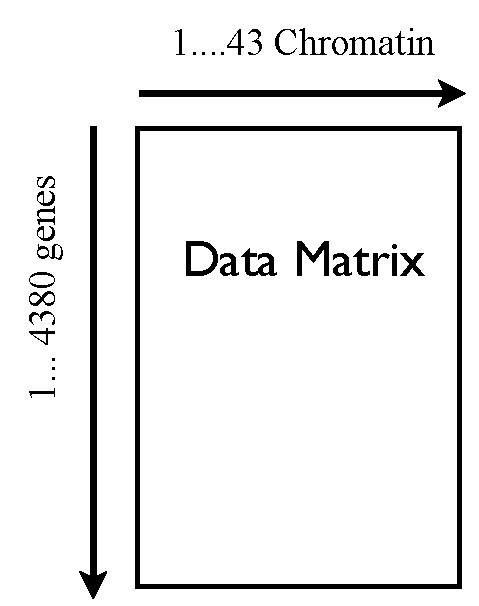
\includegraphics[width=.20\textwidth]{figures/datamatrix.pdf}
  \end{figure}
  
  \end{itemize}
}  

\frame[plain]
{
  \frametitle{Learn BN of Targeting Interactions from Scratch}
  The bootstrapping procedure (adapted from Friedman,2000)
  \begin{itemize}[<+->]
   \item For \(i = 1, ... , 1000\),
   \item Construct a slightly perturbed input data, \(D_i\), generating 1000 input data, each input data matrix has a dimension of 4380 rows each selected by random sampling with replacement from D (original dataset) and 43 columns (chromatin components)
   \item Apply the learning procedure using Banjo search on \( D_i \), generating \((G_1, ..., G_{1000})\)in total of 1000 networks.
   \item For each feature of interest compute:
   \[
   \text{Conf}(f)= \frac{1}{m} \sum_{i=1}^{m} f(G_i)\
   \]
   \[
    f(G) = \left\{ 
   \begin{array}{l l}
    1 & \quad \text{if $f$ is a feature in G}\\
    0 & \quad \text{if $f$ is absent}\\
  \end{array} \right\}
   \]


\end{itemize}
}




\section[Results]{Main Results} %summary of main results
\frame
{
 \frametitle{Reconstructed BN80}
 \begin{figure}
  \begin{center}
   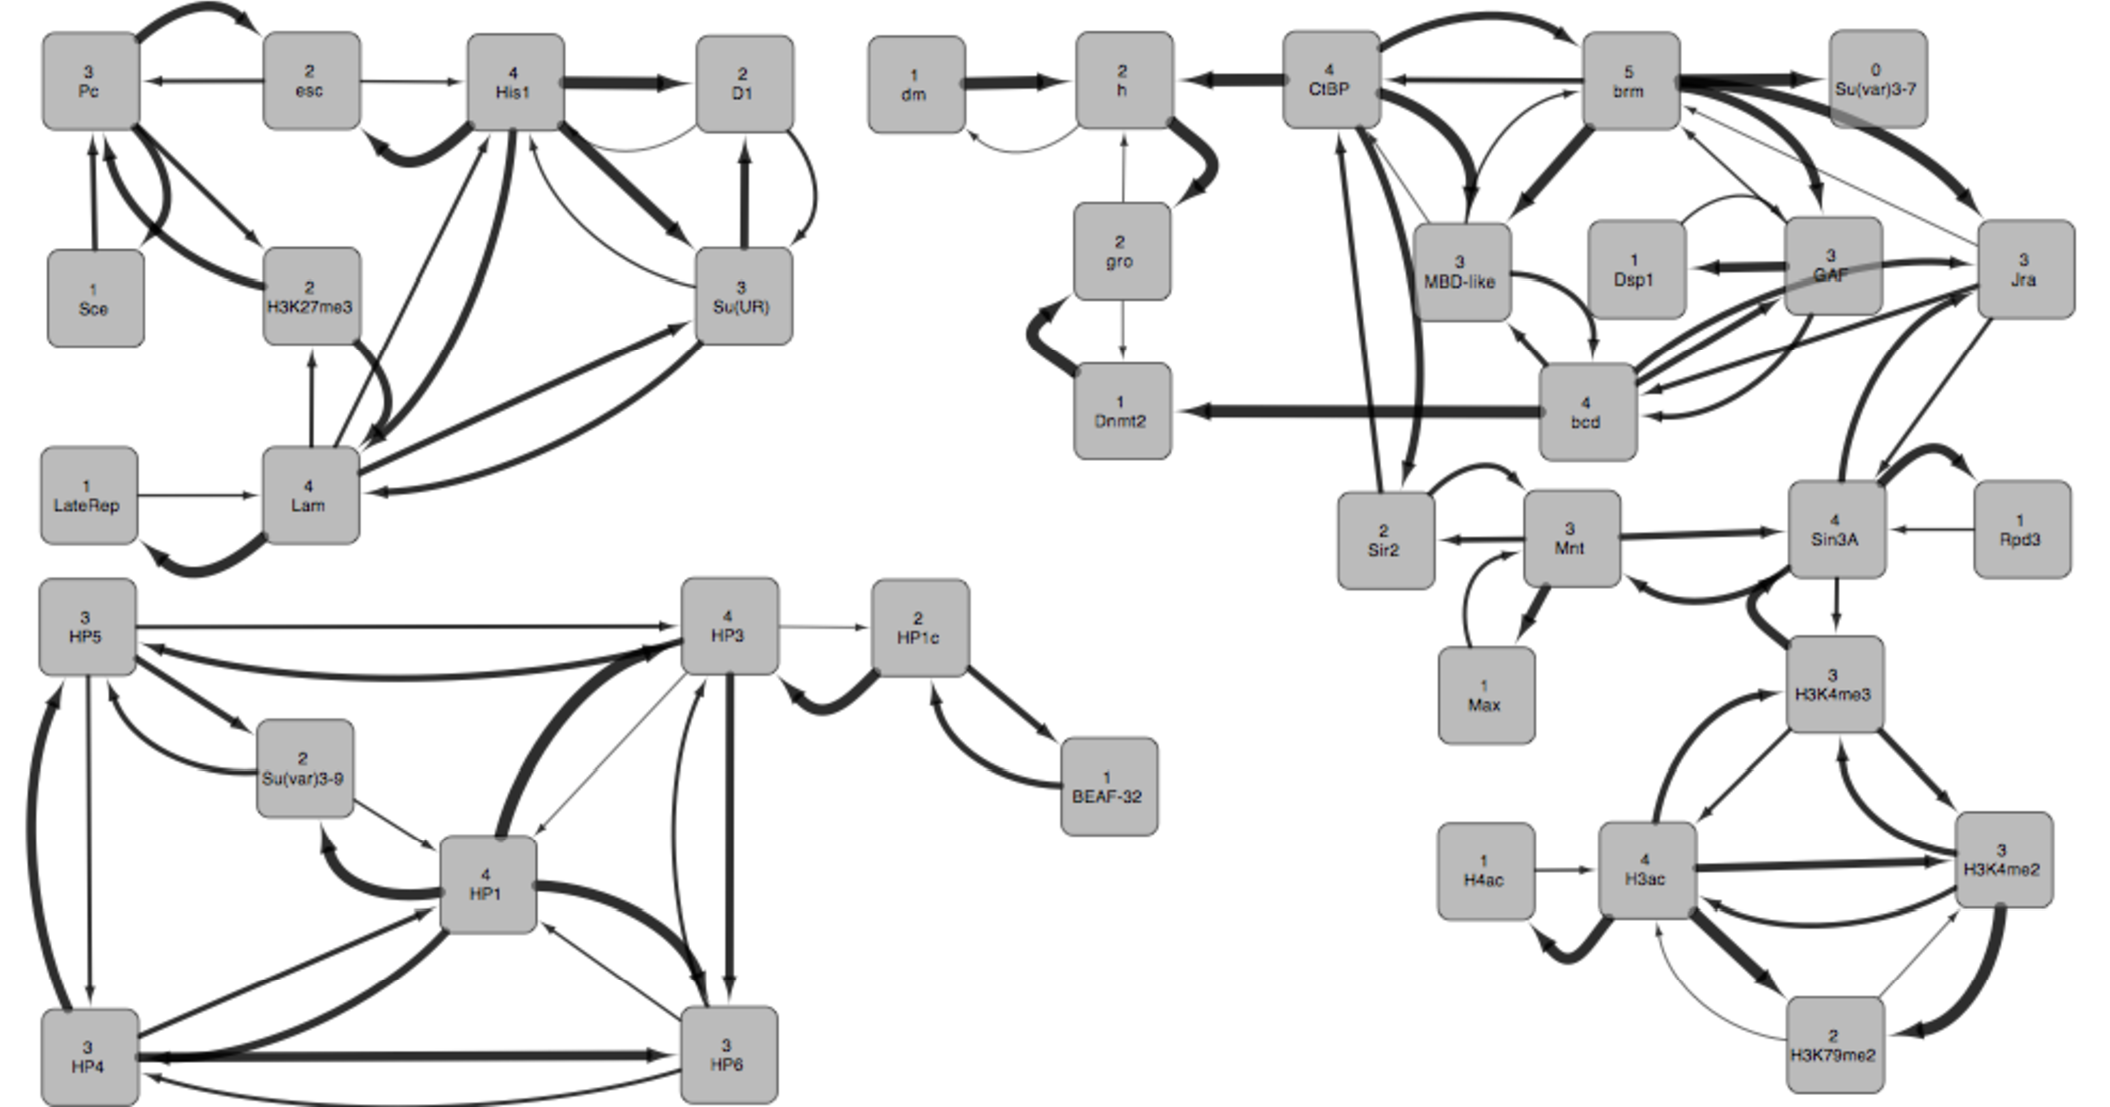
\includegraphics[width=1.05\textwidth]{figures/reconstBN80.pdf}
  \end{center}
 \end{figure}

}


\frame[plain]
{
% put text on top of the figure
 \begin{tikzpicture}[node distance = 2cm, auto,->=stealth,point/.style= 
                   {circle,fill=red,minimum size=0pt,inner sep=0pt}]
   \tikzstyle{block} = [rectangle, draw,thick,fill=blue!0,
    text centered, rounded corners, minimum height=1em]   
     
    \draw (0, 0) node[inner sep=0] {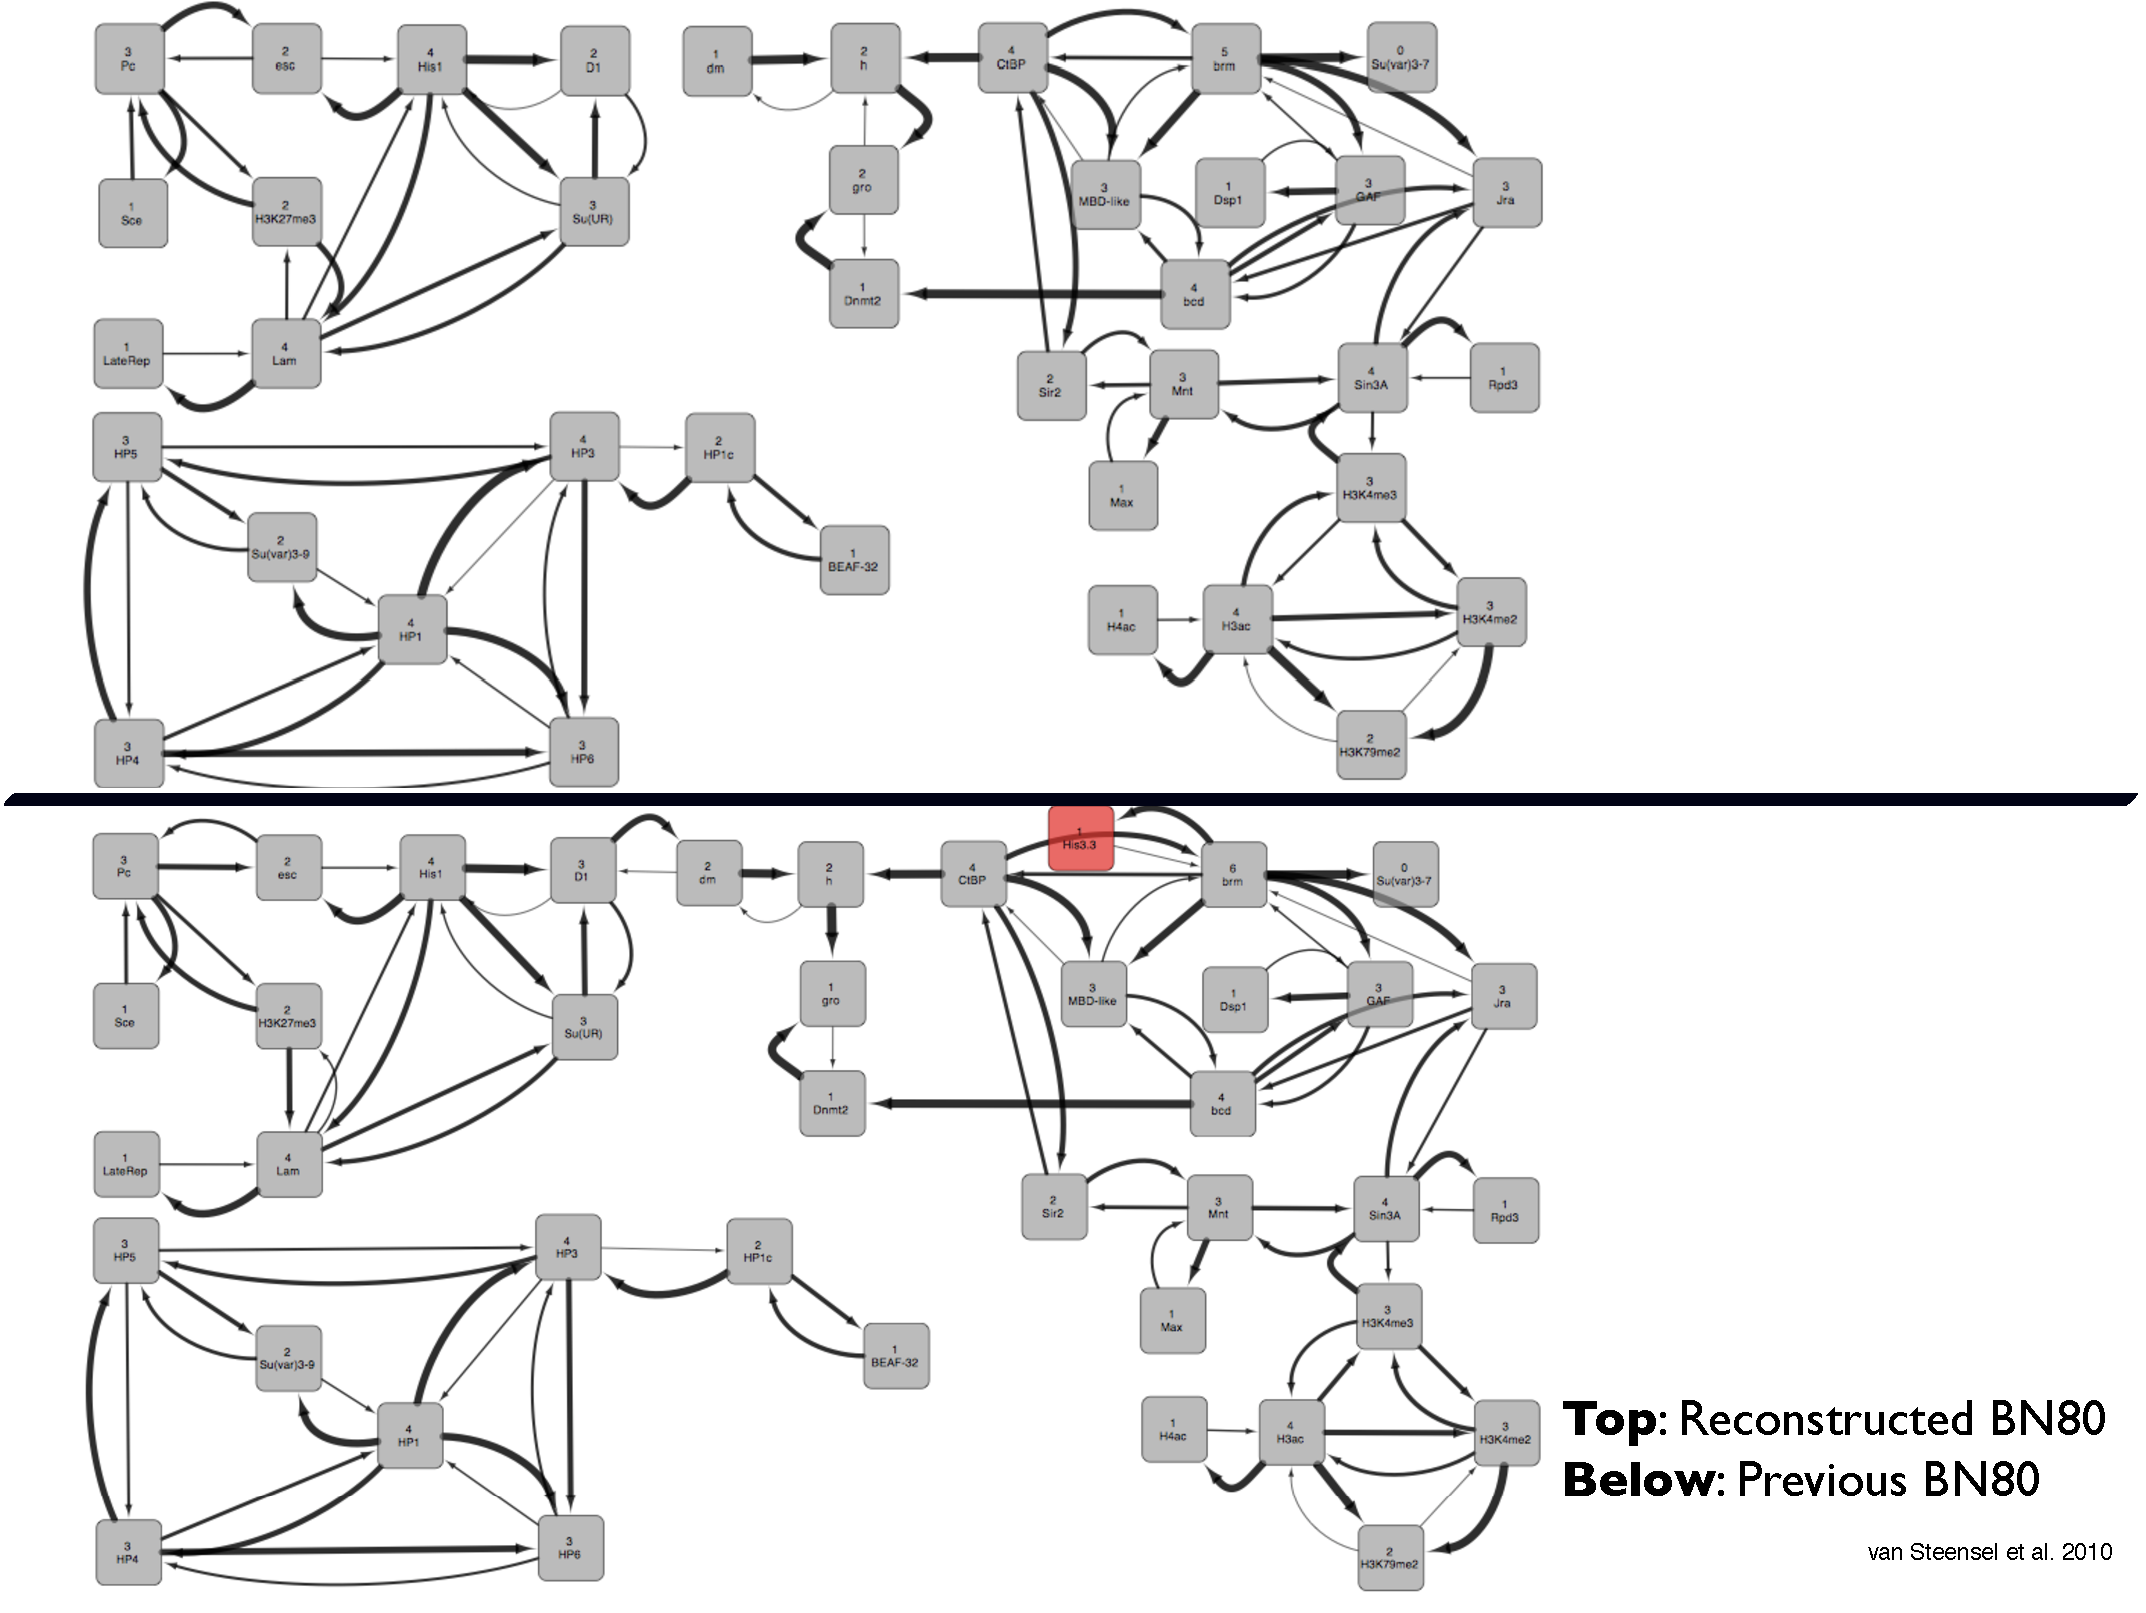
\includegraphics[width=1.1\textwidth]{figures/reconstpaperBN80.pdf}};
    \pause
    \draw (4.2, 3) node [block]  
     \end{varwidth}};
 \end{tikzpicture}
}


\frame
{
 \frametitle{BN80 Topology}
 \begin{figure}
  \begin{center}
   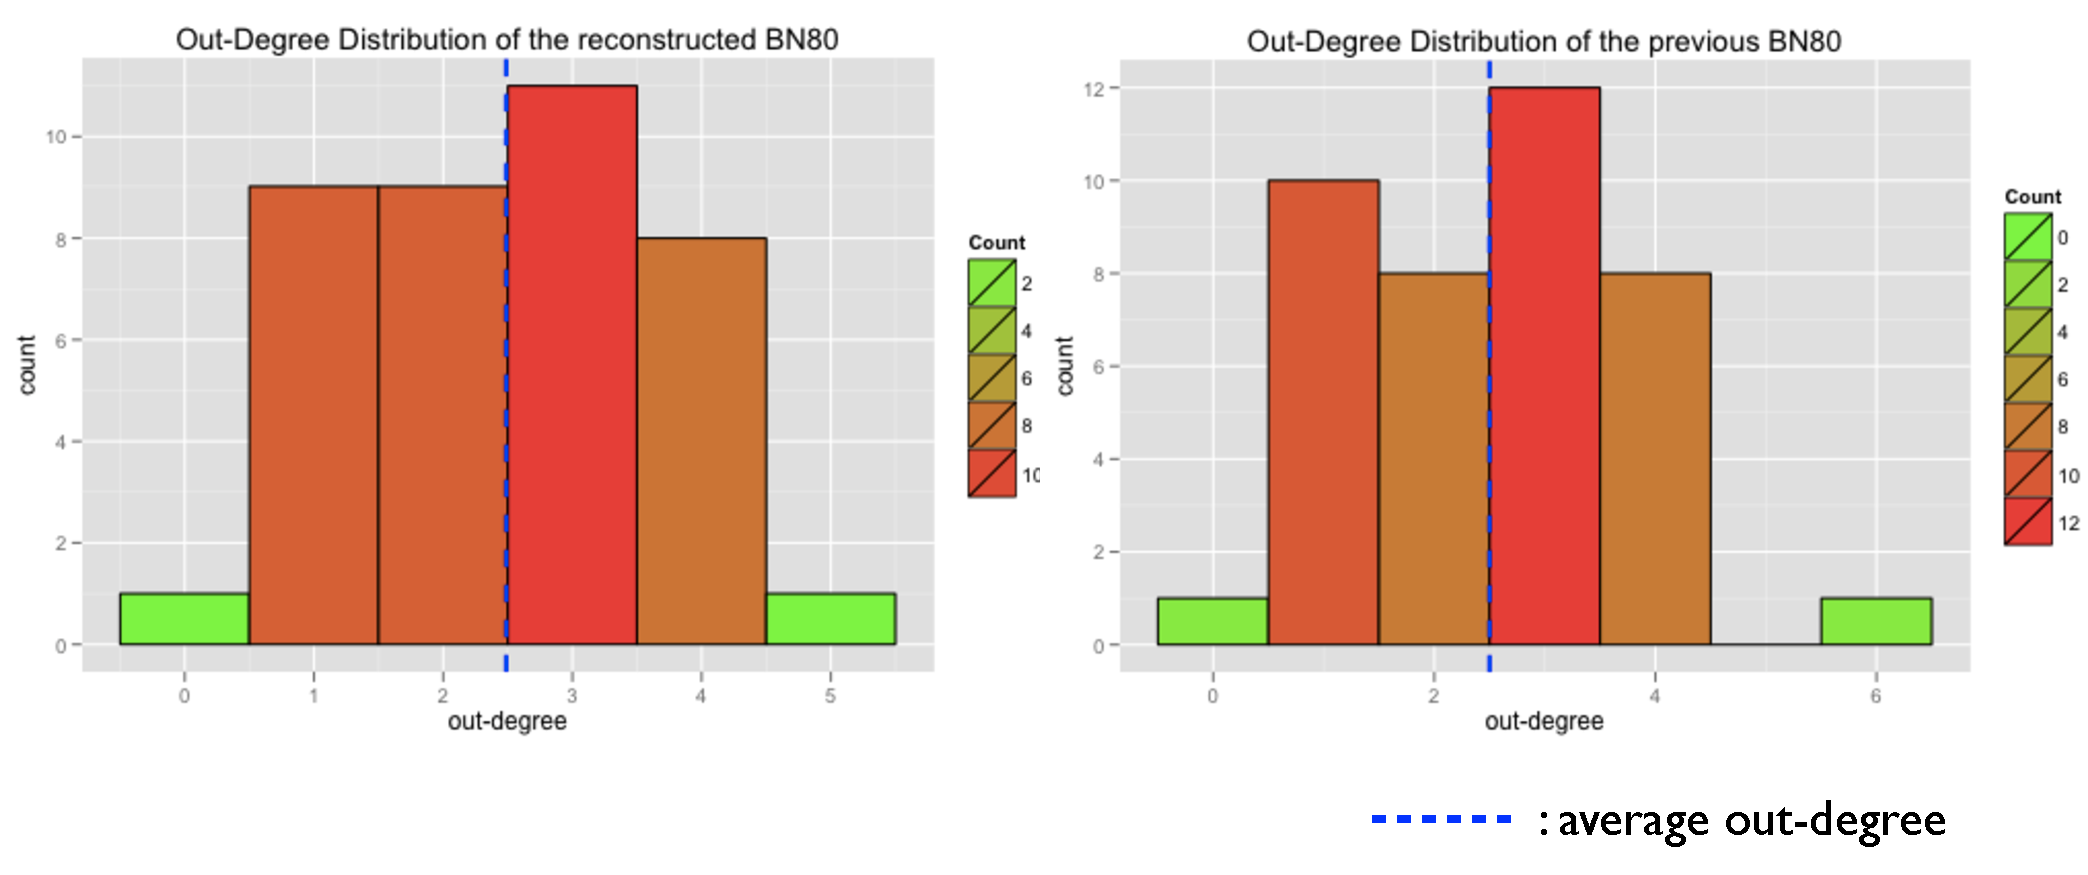
\includegraphics[width=1.05\textwidth]{figures/BN80topology.pdf}
  \end{center}
 \end{figure}
}

\frame
{
 \frametitle{PubMed Validation}
 \begin{figure}
  \begin{center}
   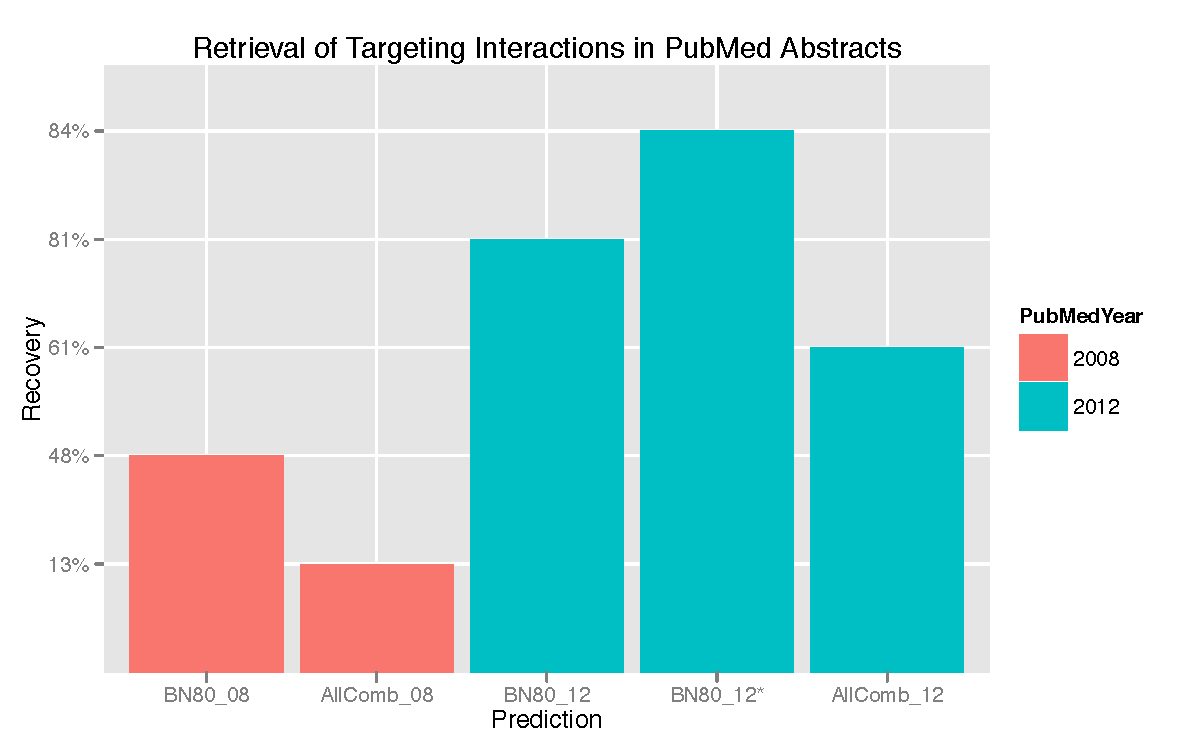
\includegraphics[width=1.0\textwidth]{figures/pubmedval.pdf}
  \end{center}
 \end{figure}
}


\section[Conclusion]{Conclusion}

\def\colorize<#1>{%
 \temporal<#1>{\color{green!50}}{\color{black}}{\color{black!50}}}
\frame
{
 \frametitle{Conclusion}
 \begin{enumerate}
  \colorize<1> \item Successfully reconstructed BN80 with the recovery rate of 96.15\% 
  \colorize<2> \item The reconstructed BN80 shares similar network topology with the average out-degree of 2.5
  \colorize<3> \item 84\% of the predicted interactions from BN80 recovered back in PubMed abstracts
 \end{enumerate}
}

\frame
{
 \frametitle{Pitfalls and Future}
 \begin{itemize}
  \colorize<1> \item Learning the causal pattern from BN is assumed that no hidden variables(i.,e no Hidden Common Cause)
  \colorize<2> \item Static BN, No feedback loops hence the temporal features are desired for the future to model dynamic BN
 \end{itemize}
}

\frame[plain]
{
 \frametitle{Acknowledgment}
 \begin{itemize}
  \item Gunnar W. Klau
  \item Alexander Schoenhuth
  \item Guillaume Filion
  \item Tycho Bismeijer
 \end{itemize}
}

\frame[plain,allowframebreaks]
{
 \frametitle{References}
1.	van Steensel B, Braunschweig U, Filion GJ, Chen M, van Bemmel JG, et al. (2010) Bayesian network analysis of targeting interactions in chromatin. Genome Research 20: 190–200. doi:10.1101/gr.098822.109.

2.	Horn PJ (2002) MOLECULAR BIOLOGY: Chromatin Higher Order Folding--Wrapping up Transcription. Science 297: 1824–1827. doi:10.1126/science.1074200.

3.	Rando OJ, Chang HY (2009) Genome-wide views of chromatin structure. Annu Rev Biochem 78: 245–271. doi:10.1146/annurev.biochem.78.071107.134639.

4.	Pe'er DD (2005) Bayesian network analysis of signaling networks: a primer. CORD Conference Proceedings 2005: pl4–pl4.

5.	Friedman N, Linial M, Nachman I, Pe'er D (2000) Using Bayesian networks to analyze expression data. J Comput Biol 7: 601–620. doi:10.1089/106652700750050961.

6.	Heckerman D (n.d.) A tutorial on learning with bayesian networks. researchmicrosoftcom.\\
Available:http://research.microsoft.com/pubs/69588/tr-95-06.pdf.\\
Accessed 21 February 2012.

7.	Oufir EA (n.d.) Suitability of Bayesian Networks for the Inference and Completion of Genetic Networks using Microarray Data. Voorbraak F, Visser A, editors Amsterdam: science.uva.nl. pp.

8.	Vesterstrøm J (n.d.) Heuristic Algorithms in Bioinformatics. daimi.au.dk. pp.

9.	Cline MS, Smoot M, Cerami E, Kuchinsky A, Landys N, et al. (2007) Integration of biological networks and gene expression data using Cytoscape. Nat Protoc 2: 2366–2382. doi:10.1038/nprot.2007.324.

10.	Chavan SS, Bauer MA, Scutari M, Nagarajan R (2009) NATbox: a network analysis toolbox in R. BMC Bioinformatics 10 Suppl 11: S14. doi:10.1186/1471-2105-10-S11-S14.
}

\appendix
\section{DAM-ID: Mapping Method}
\frame[label=damid]
{
 \frametitle{DAM-ID: Mapping Method}
 \FrameText{\hfill\hyperlink{map}\insertreturnsymbol}
 \begin{figure}
  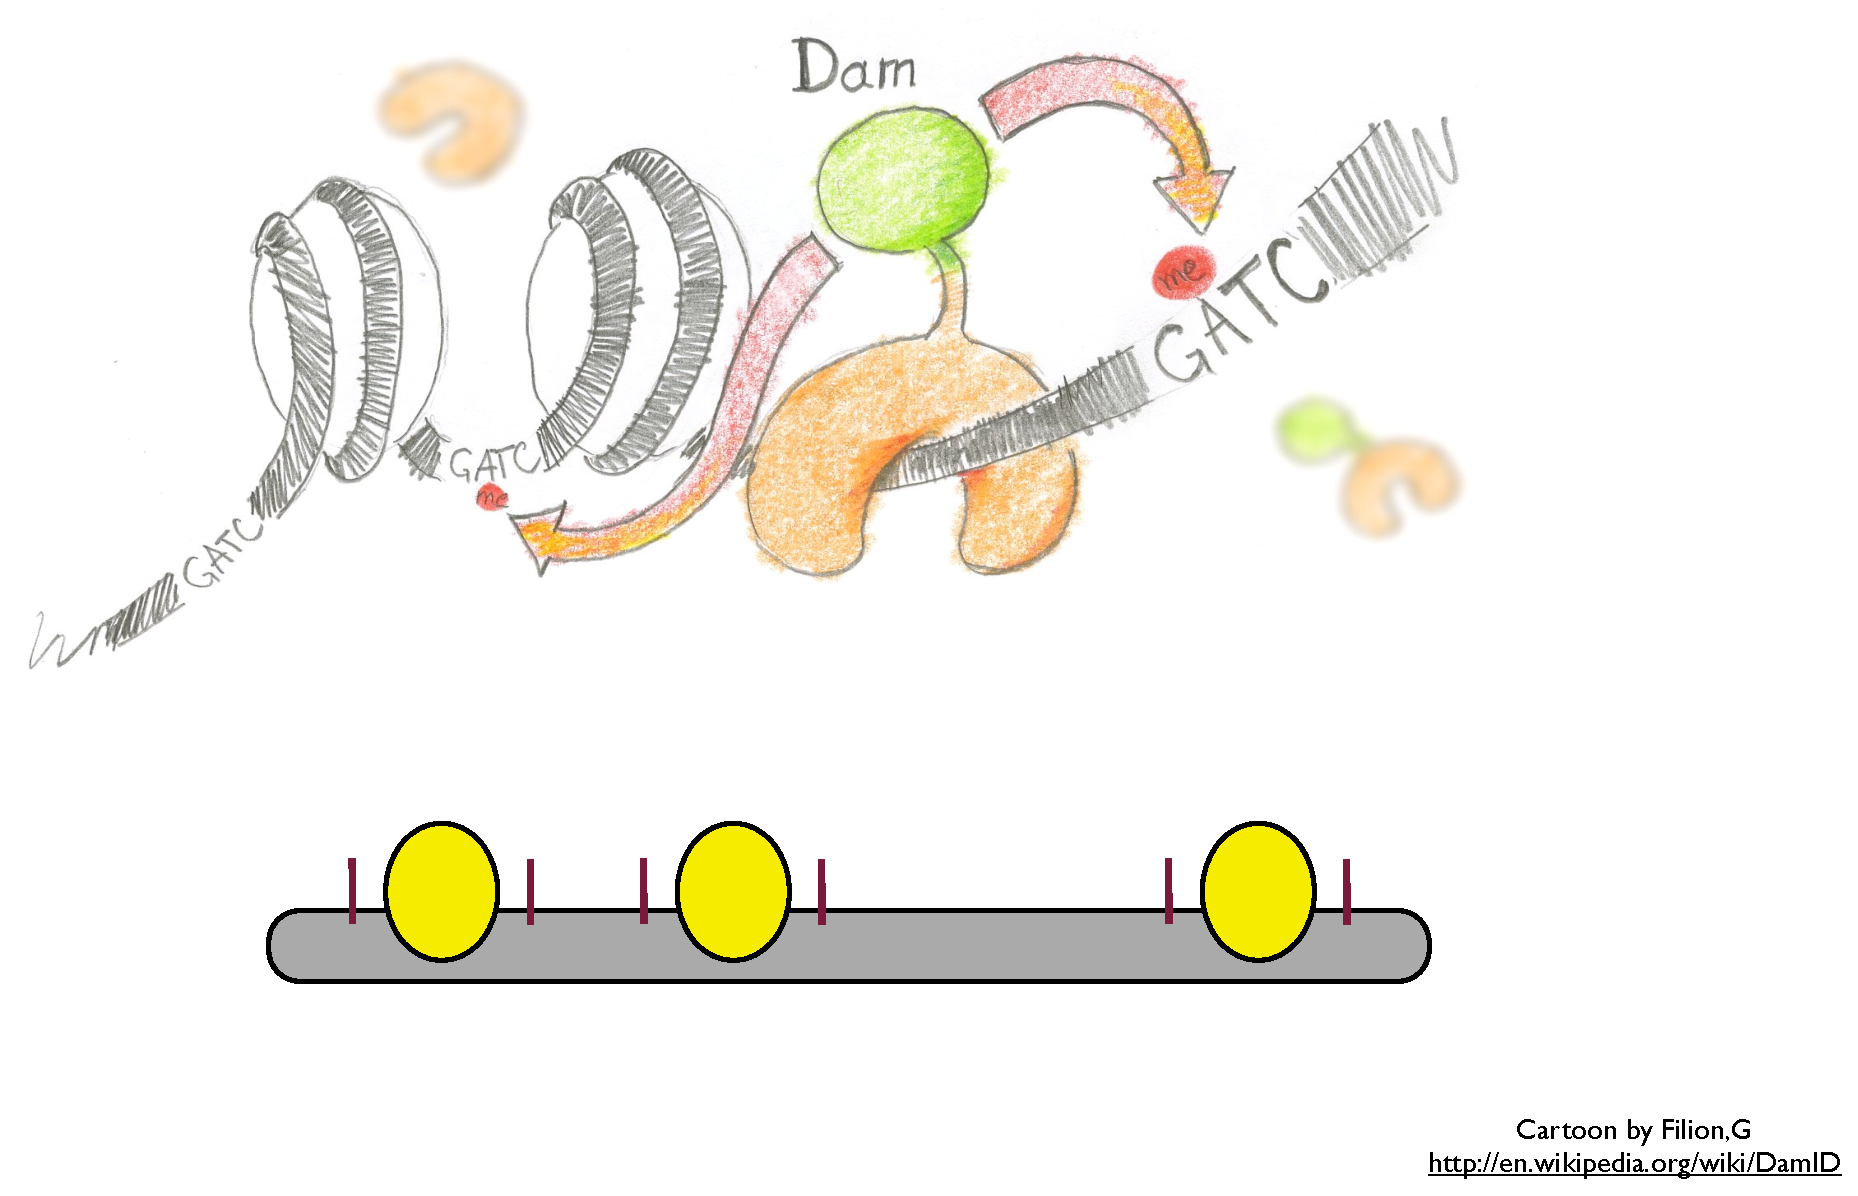
\includegraphics[width=.9\textwidth]{figures/damid.pdf}
 \end{figure}
 
}


\frame[plain]
{
 \frametitle{DAM-ID: Mapping Method}
 
 \begin{minipage}{0.50\textwidth}
  \begin{figure}
   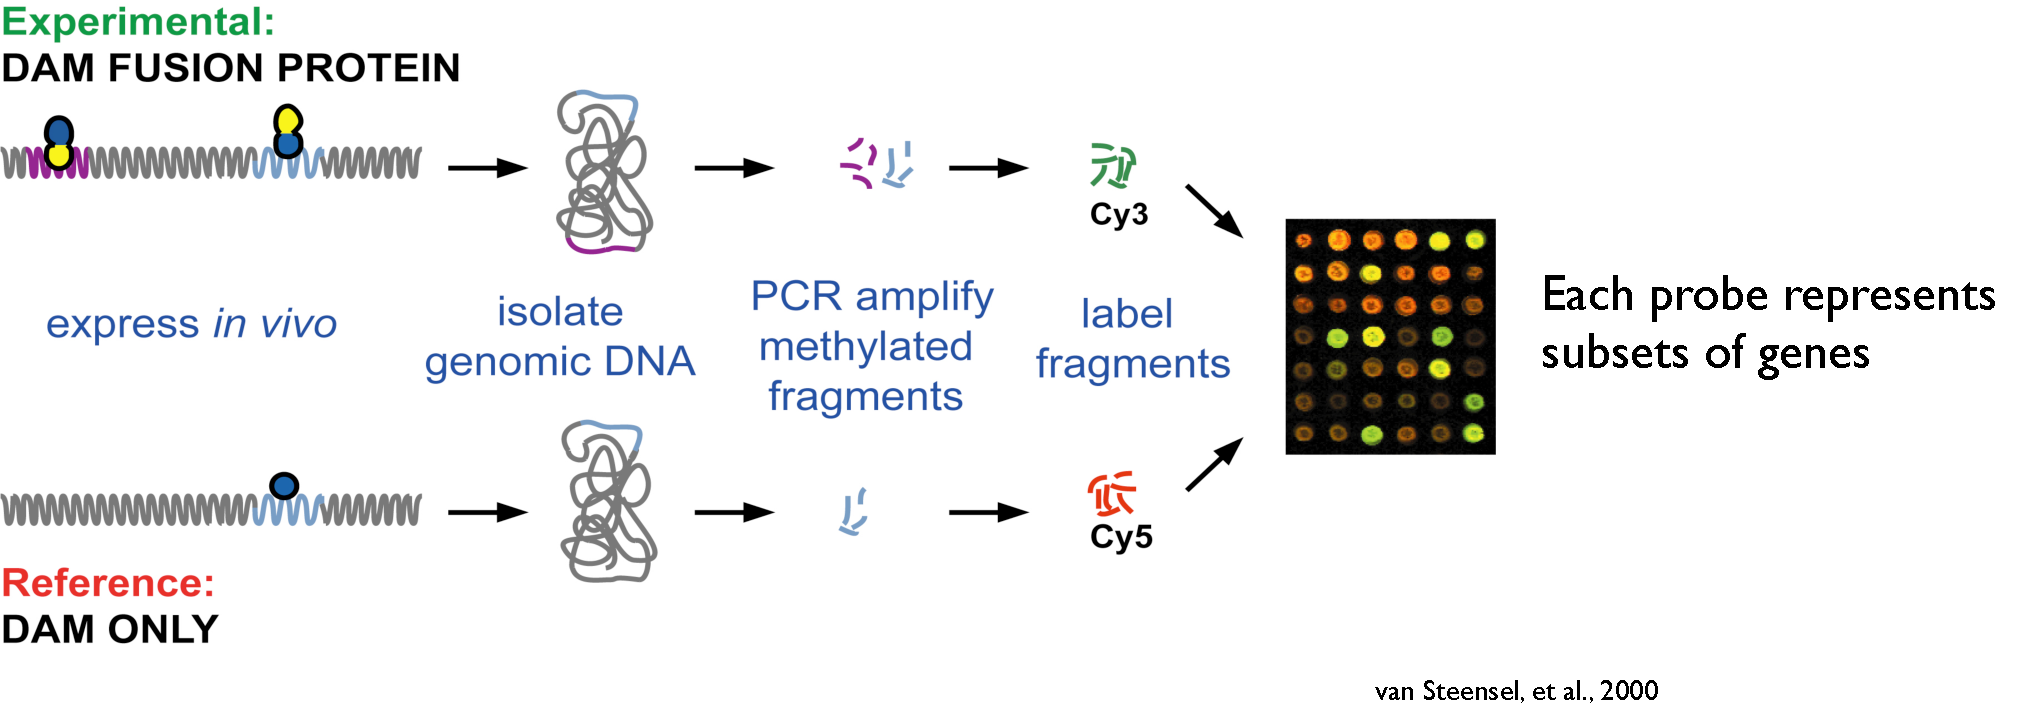
\includegraphics[width=2.1\textwidth]{figures/damidprot.pdf}
  \end{figure}
 \end{minipage}
 \pause
 \begin{minipage}[t]{0.50\textwidth}
   \begin{minipage}[t]{0.4\textwidth}
    \vspace{0pt}
    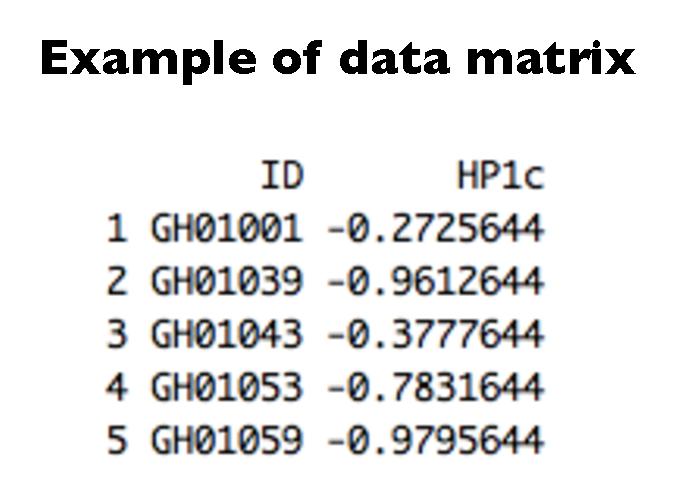
\includegraphics[width=1.5\textwidth]{figures/damidmatrix.pdf}
   \end{minipage}
   \hfill
   \pause
   \begin{minipage}[t]{0.5\textwidth}
    \vspace{0pt}
    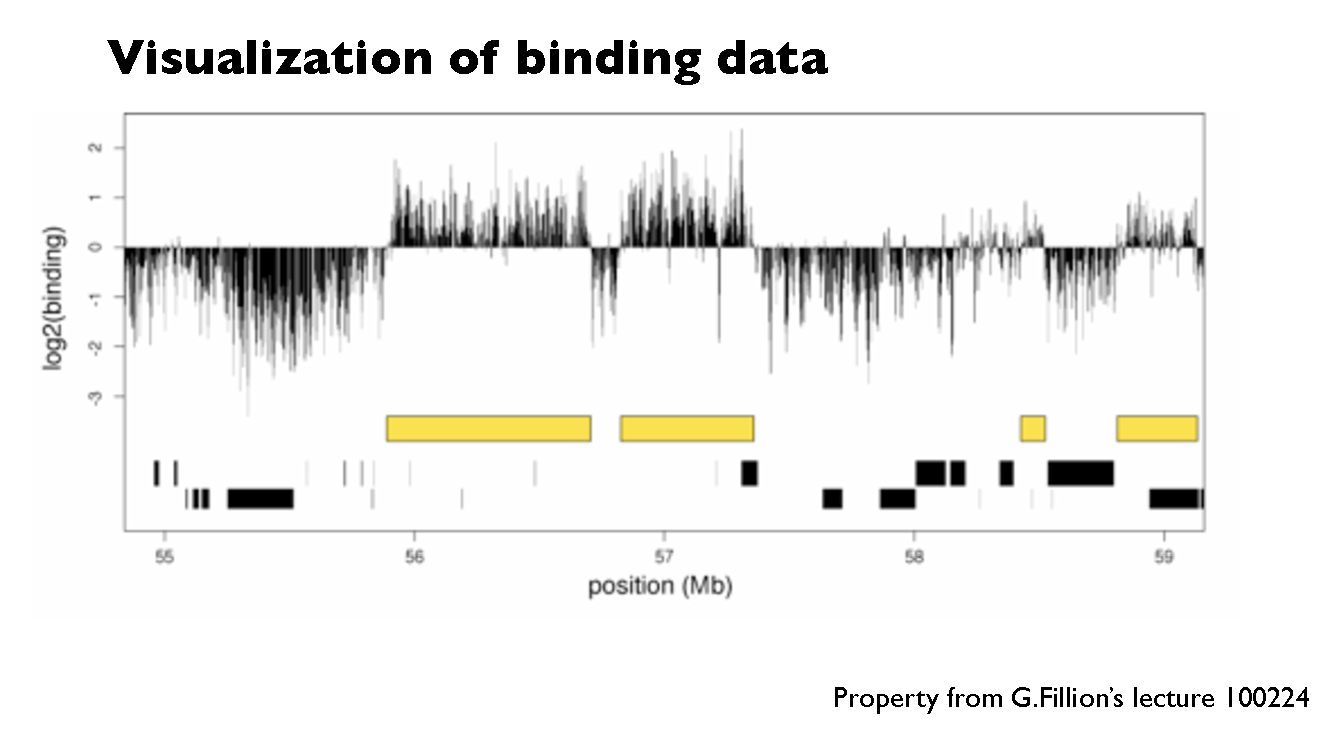
\includegraphics[width=2.7\textwidth]{figures/damidvisual.pdf}
   \end{minipage}
 \end{minipage}
}


\end{document}
